\documentclass{article}
% \usepackage[margin=2.5cm]{geometry}
\usepackage[margin=2.5cm, headheight=0pt, headsep=1cm]{geometry}
\usepackage{enumerate, fancyhdr, graphicx, amsmath, nth}
\usepackage[binary-units=true]{siunitx}

\title{Big Brother Is Watching}
\author{Paul Chesnais (pmc85), Nimit Sohoni (nss66) and Matthew Siebert (mrs345)}
\date{\today}

\pagestyle{fancy}
\fancyhead{}
\lhead{pmc85, nss66 and mrs345}
\chead{Big Brother}
\rhead{\today}
\fancyfoot{}
\rfoot{\thepage}
\lfoot{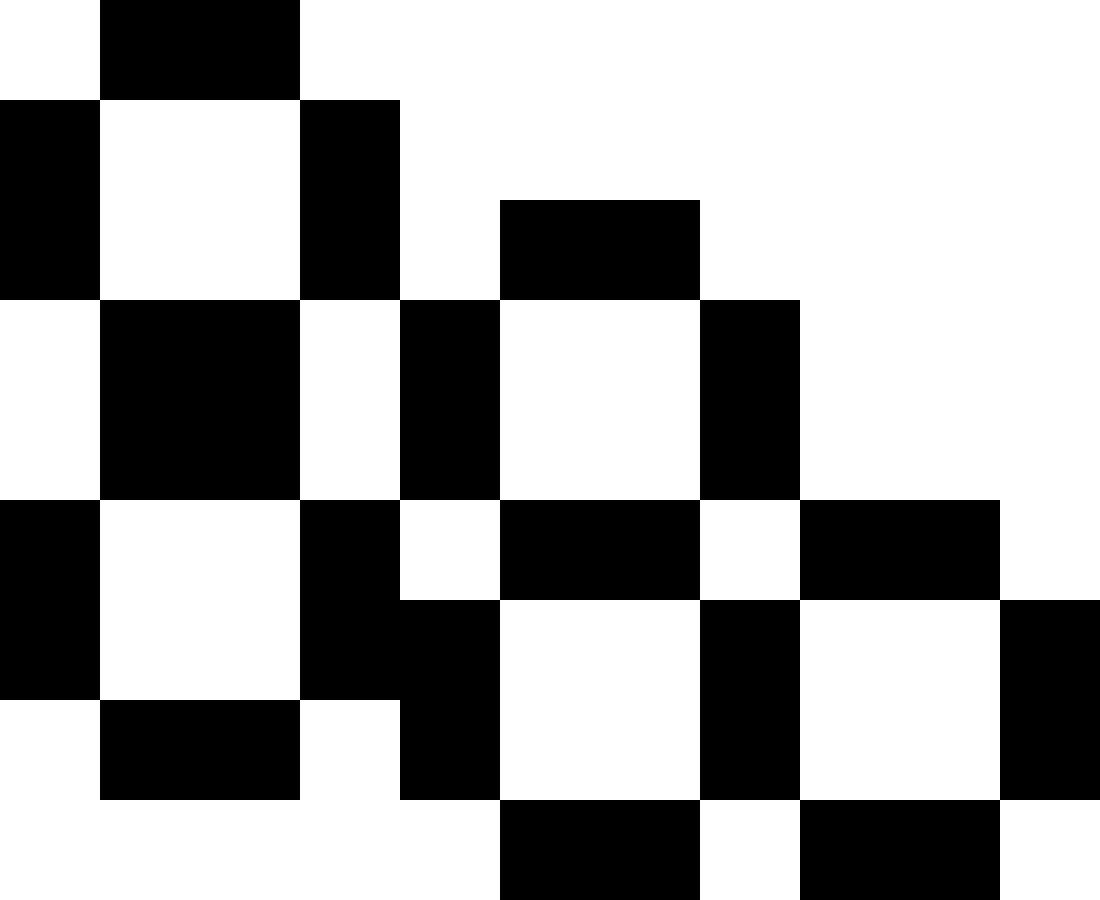
\includegraphics[height=20pt]{Logo}}
\renewcommand{\headrulewidth}{0.5pt}
\renewcommand{\footrulewidth}{0.5pt}

\DeclareSIUnit{\mph}{mph}

\usepackage{listings, color, times, textcomp, float, hyperref, subcaption}
\definecolor{mygreen}{RGB}{28,172,0} % color values Red, Green, Blue
\definecolor{mylilas}{RGB}{170,55,241}
\lstset{language=Matlab, basicstyle=\scriptsize\ttfamily,breaklines=true,
frame=single,morekeywords={matlab2tikz},keywordstyle=\color{blue},
morekeywords=[2]{1},keywordstyle=[2]{\color{black}},
identifierstyle=\color{black},stringstyle=\color{mylilas},
commentstyle=\color{mygreen},showstringspaces=false, numbers=left,
numberstyle={\tiny \color{black}},numbersep=9pt,emph=[1]{for,end,break},
emphstyle=[1]\color{red},literate={~} {\texttildelow}{1}}

\newcommand{\exo}[1]{\section*{Exercise #1}}
\newcommand{\prob}[1]{\section*{Problem #1}}
\newcommand{\quest}[1]{\section*{Question #1}}
\newcommand{\e}{&=&}
\newcommand{\p}[1]{\times 10^{#1}}

\begin{document}
\maketitle
\thispagestyle{empty}

\section{Abstract}
\label{sec:abstract}


\section{General Assumptions}
\label{sec:general_assumptions}
\paragraph{Representing Manhattan}
\label{par:representing_manhattan}
First, we want to justify our representation of Manhattan. Manhattan is a long thin strip of land, spanned vertically by \emph{avenues} and horizontally by \emph{streets}. Manhattan is effectively 250 streets long, and 10 avenues wide. A Manhattan city block is \SI{80}\m by \SI{274}\m. We can approximate Manhattan, or at least this hypothetical version of Manhattan as part of Gotham City, to be a grid 250 blocks long by 30 blocks wide, where a block is an arbitrary unit of distance, in this case \SI{80}\m. In this representation, Central Park is 10 blocks wide and 51 blocks long, since the real Central Park is 3 avenues wide and goes from \nth{59} Street to \nth{110} Street, occupying the middle 3 avenues \cite{centralpark}. Similarly, if we take Gotham University to be the fictional equivalent of Columbia University, which is found between \nth{110} Street and \nth{122} Street and spans the 3 westernmost avenues of Manhattan \cite{columbia}, then we can it to be an area 12 block long and 9 blocks wide. Finally, the Financial District is contained in the southernmost 20 streets in Manhattan \cite{financial}, hence we can make it occupy the last 20 rows in our matrix.

\paragraph{Representing Time}
\label{par:representing_time}
Next, we also justify our representation of time. Instead of modeling it as a continuous variable, it is better to model it as discrete steps in time, where drones can move a fixed distance and observe a fixed number of blocks per step. For simplicity, we will make these steps in time exactly one minute long.

\paragraph{Drone Speed}
\label{par:drone_speed}
Recent legislation has limited the speed of drones at \SI{100}\mph \cite{dronespeed}. Having drones zipping around Manhattan at \SI{100}\mph seems not only dangerous, it seems that they would not be able to gather very meaningful data. As such, for the purposes of this simulation, we made our drones relatively slow and limited the to a speed of 10 blocks per minute.

\paragraph{Drone Sight}
\label{par:drone_sight}
For this particular fictional reality, we assume that drones need to take pictures of the jaywalkers' faces in order to flag them. As such, we assume in a drone can only see jaywalkers in the intersection it is currently hovering over. This means that a drone needs to physically fly over a particular intersection for it to be counted as ``visited''.

\section{Simplifications}
There are two simplifications that we reserved the right to make when designing our strategies. They make the solutions more elegant and easier to compute, while not preventing us from then generalizing our optimal solutions back to the original problem.
\paragraph{Flight and Recharge Time}
\label{par:flight_and_recharge_time}
One parameter that was made unclear is once drones run out of fuel, how long does it take them to recharge? Suppose we have an optimal solution that requires exactly $n$ drones. If it takes a drone exactly 5 hours to recharge, and we need to keep $n$ drones in the air at all times, then we need a minimum of $2n$ drones to guarantee our ability to do so. Similarly, if the time to recharge is 1 hour, then we can interleave the drones' schedules such that one drone goes down every hour, and we only need $n+1$ drones to achieve the optimal solution. There is an inverse relationship between the amount of time it takes to recharge the drones (relative to the amount of time a drone can stay in the air), and the total number of drones needed to achieve a particular solution. As such, we can begin by finding an optimal solution requiring $n$ drones where drones can fly indefinitely, then fine tuning $n$ with regards to the flight and recharge time constraints accordingly.
\paragraph{Charging Stations}
\label{par:charging_stations}
Another consideration for this summation may be that the drones can only be launched from a limited number of charging stations. Suppose a strategy involves splitting up Manhattan into quadrants, then assigning drones for each quadrants. If drones can only launch from certain locations within Manhattan, they may take some time to get their respective areas, which may lead to lost observation time. There are two reasons why the following models do not take this into account. First of all, in the grand scheme of the strategy, what matters is what happens in the majority of the time, not the small amount of time it takes for the drone to move to its area, relative the total amount of time the drone is in the air. The other reason is that while the speed of our drones is 10 blocks per minute while watching for jaywalkers, nothing was said about their actual top speed. There is reason to believe that if a \SI{100}\mph speed limit exists, some drones are capable of reaching that speed, and will indeed do so if required while relocating to a new quadrant. Therefore we can assume that drones ``spawn'' in the correct location at the beginning of time.

% Matt's stuff n' things
\section{Optimal Path Model}
\label{sec:optimal_path_model}

% Nimit's stuff and things
\section{Block Model}
\label{sec:block_model}

% Paul's stuff n' things
\section{Greedy Random Walk}
\label{sec:greedy_random_walk_model}
Since some fellow jaywalkers don't want us to have an advantage when walking the in the streets of Manhattan, we also need a strategy that is a little more unpredictable. Part of the problem with the strategies outlined above is that knowing the location of a single drone lets someone with inside knowledge about the strategy infer the location of every other drone, or at least the location of neighboring drones. One response to this complaint would be to make the drones travel a more random path. The following strategy does just that, and works even when areas of Manhattan have different densities of jaywalkers.

\subsection{Global State}
\label{sub:global_state}
One of the requirements of this strategy is that a global state accessible by all drones is required. It seems reasonable to assume that cellphone networks still exist in 2084, and therefore that all of our drones are connected to the Internet. Two pieces of information need to be kept about each node in the grid: the time at which the node was last visited, and the required frequency at which it needs to be watched.

\subsection{Greedy walk}
\label{sub:greedy_walk}
As mentioned above, drones have access to the timestamp of the last visit for a given intersection, and the amount of time that can pass before said intersection needs to be watched again. As such, the ``urgency'', or how soon a given node must be visited, can be inferred.

\section{Conclusion}
\label{sec:conclusion}


\section{Appendix}
\label{sec:appendix}

\subsection{Greedy Walk Source}
\label{sub:greedy_walk_source}
\lstinputlisting{models/random_movement.m}
\lstinputlisting{models/MAV.m}

\begin{thebibliography}{9}
  \bibitem{columbia}
    \url{https://www.google.com/maps/place/columbia+university/@40.8075355,-73.9625727,15z/data=!4m2!3m1!1s0x0:0x577933f947e52750?sa=X&ved=0CIcBEPwSMBdqFQoTCMay2Oi09cgCFQJ4Jgod360LJA}
  \bibitem{financial}
    \url{https://www.google.com/maps/place/Financial+District,+New+York,+NY/data=!4m2!3m1!1s0x89c25a18338ac807:0x2bac148b119ab3?sa=X&ved=0CIUBEPIBMA1qFQoTCKr37smw9cgCFUJkJgodYywMtA}
  \bibitem{centralpark}
    \url{https://www.google.com/maps/place/Central+Park,+New+York,+NY/@40.7828647,-73.9653551,15z/data=!4m2!3m1!1s0x89c2589a010bc7f5:0xc159962ffd2019b6}
  \bibitem{dronespeed}
    \url{http://www.npr.org/sections/thetwo-way/2015/02/15/386464188/commercial-drone-rules-to-limit-their-speed-and-altitude}
\end{thebibliography}


\end{document}